\section{Das Allerbeste zum Schluss: Ausgew\"ahlte Ereignisse in und um Granitz}
\label{sec:events}

Bis hierhin ging es nur um die Erstellung der Anlage sowie ihre Technik.
Es w\"are zu schade, die Einblicke in das eigentliche Geschehen in Granitz und Umgebung auszusparen.
Das regul\"are Betriebsgeschehen sowie Tage, an denen ungew\"ohnlich viele Schaulustige an den Streckenr\"andern stehen, laden zu einer losen Sammlung von Geschichten ein.
Insbesondere im Bild soll hier festgehalten werden, wann Granitz wie aussah, was sich \"uber die Zeit ge\"andert hat.
Und es sollen Gastauftritte von Z\"ugen gezeigt werden, die au{\ss}erplanm\"a{\ss}ig die Brandenburger Heiden durchqueren.

Insgeheim hoffe ich nat\"urlich, dass dieses Kapitel das sch\"onste wird.
Fernab aller vorheriger Planungen wird hier auch der jeweilige Ist-Zustand auf einem Zeitstrahl verewigt.
Die Z\"uge sind in Aktion, das Diorama peu a peu belebt.
Ich freue mich auf die kontinuierliche Erweiterung!


\subsection{Spatenstich und Erstfahrten}
\label{sec:firstNail}

Erg\"anzend zum historischen Abriss aus der Einleitung sollen an dieser Stelle rare Zeitdokumente pr\"asentiert werden.
Wie so oft, ist das Kramen in den Archiven m\"u{\ss}ig und es gibt aus den Anfangstagen von Granitz - das f\"uhrt ins ins 19. Jahrhundert zur\"uck! - nicht viel Fotomaterial.

Abbildung~\ref{img:events_first_nail} zeigt den Spatenstich zu den Gleisbauarbeiten in Granitz.
Irgendein Gr\"u{\ss}august, ggf. der damalige B\"urgermeister, schlug den ersten Nagel durch eine Schienenschwelle in der Granitzer Gleisw\"uste.
Das Datum ist unbekannt.
Allein die Digitalisierung des Bildes fand am 19. April 2020 um Punkt 18:00 Uhr (CEST) statt.
Hingegen ist der Ort auch noch heute gut auszumachen:
Wir befinden uns an der Westeinfahrt von Granitz, konkret an der Eingangsweiche, die von Gleis III den Wechsel auf Gleis V bereitstellt.

\begin{figure}[h]
\centering
  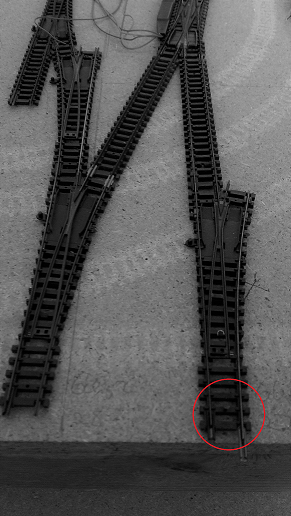
\includegraphics[width=0.3\textwidth]{img/events/first_nail_edit.png}
	\caption{Erster Nagelschlag an der Westeinfahrt von Granitz}
	\label{img:events_first_nail}
\end{figure}

\clearpage

\hl{Die erste richtige Fahrt erfolgte.....}



\subsection{Event I ...}

\subsection{Event II ...}

\subsection{Event III ...}